\chapter{Måling på HiFi-forstærker}
\label{maaling_hifi}
Denne målerapport dokumenterer målinger foretaget på projektets HiFi-forstærker, opbygget som beskrevet igennem hele rapporten. Målingerne er foretaget på Fredrik Bajers Vej 7 i lokale B1-104 på Aalborg Universitet den 20. december 2010 af gruppe 311.

\section*{Formål}
Målingernes formål er at teste:

\begin{itemize}
\item Frekvensgangen fra 20 Hz - 20 kHz
\item Forvrængningen
\item Forstærkning
\end{itemize}

\section*{Testobjekt}
Målingerne udføres på projektets samlede HiFi-forstærkeren. Diagrammet for denne findes i bilag \kilde{bilag med high-def diagram af det hele}.

\section*{Måleopstilling}
Målingerne foretages   ved en opstilling, der laver forstærkning-, frekvensgang- og forvrængningsmåling. Opstillingen er vist på figur \ref{fig:maaleop-hifi}.

\begin{figure}[h]
\centering
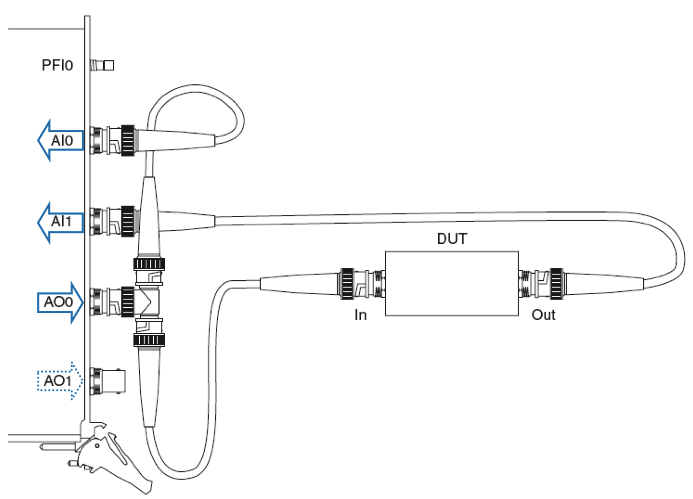
\includegraphics[scale=0.3]{maalerapporter/forforstaerker/maaleopstilling-thd-forforstaerker.png}
\caption{Måleopstilling for forstærkning-, frekvensgang- og forvrængningsmåling \cite{maaling-mm5}}
\label{fig:maaleop-hifi}
\end{figure}

\section*{Anvendt udstyr}

\begin{table}[h]
\centering
\begin{tabular}{l|c|l}
\hline\hline
Instrument & AAU-nr. & Fabrikant, type m.v. \\
\hline\hline
Spændingsforsyning & 33898 & HAMEG HM7042 \\[4pt]
Spændingsforsyning & 33907 & HAMEG HM7042 \\[4pt]
Spændingsforsyning & 33904 & HAMEG HM7042 \\[4pt]
Multimeter & 08517 & Fluke and Philips FLUKE 37 \\[4pt]
Audioanalysator & 76986  & National Instruments NI-PCI-4461 \\[4pt]
Effektmodstand & 2159-04 & 8,2 \ohm \\
\hline\hline
\end{tabular}
\label{tab:maaleudstyr_hififorstærker}
\end{table}

\section*{Måleprocedure}
Proceduren for forstærkning-, frekvensgang- og forvrængningsmålingen, på stereo indgangen, er:

\begin{enumerate}
\item En spændingsforsyning indstilles til $\pm$23 V (indstilles med multimeteret) og tilsluttes.
\item En spændingsforsyning indstilles til $\pm$15 V (indstilles med multimeteret) og tilsluttes.
\item En spændingsforsyning indstilles til 5 V (indstilles med multimeteret) og tilsluttes.
\item Testobjektet tilsluttes som på figur \ref{fig:indgang:maaleop-thd}
\item Kanalen der måles på, indstilles ved hjælp af trykknappen.
\item Programmet $"$Swept Sine - Linear Response and Harmonic Distortion (DAQmx)$"$ startes
\item $"$Start frequency$"$ under Source settings sættes til 20 Hz
\item $"$Stop frequency$"$ under Source settings sættes til 20 kHz
\item $"$Amplitude$"$ under Source settings sættes til 2 V
\item $"$THD units$"$ sættes til \%
\item $"$AI Range$"$ for Stimulus channel sættes til $\pm$3,16 V
\item $"$AI Range$"$ for Respons channel sættes til $\pm$31,6 V
\item $"$Sampling frequency$"$ sættes til 204,8 kHz
\end{enumerate}

Proceduren for forstærkning-, frekvensgang- og forvrængningsmålingen, på mikrofonindgangen, er:

\begin{enumerate}
\item En spændingsforsyning indstilles til $\pm$23 V (indstilles med multimeteret) og tilsluttes.
\item En spændingsforsyning indstilles til $\pm$15 V (indstilles med multimeteret) og tilsluttes.
\item En spændingsforsyning indstilles til 5 V (indstilles med multimeteret) og tilsluttes.
\item Testobjektet tilsluttes som på figur \ref{fig:indgang:maaleop-thd}
\item Kanalen der måles på, indstilles ved hjælp af trykknappen.
\item Programmet $"$Swept Sine - Linear Response and Harmonic Distortion (DAQmx)$"$ startes
\item $"$Start frequency$"$ under Source settings sættes til 20 Hz
\item $"$Stop frequency$"$ under Source settings sættes til 20 kHz
\item $"$Amplitude$"$ under Source settings sættes til 2 V
\item $"$THD units$"$ sættes til \%
\item $"$AI Range$"$ for Stimulus channel sættes til $\pm$0,316 V
\item $"$AI Range$"$ for Respons channel sættes til $\pm$31,6 V
\item $"$Sampling frequency$"$ sættes til 204,8 kHz
\end{enumerate}

\section*{Resultater}

THD, frekvensgang og forstærkning blev målt for de forskellige opsætninger. Resultaterne for THD vises på figur \ref{maalerapport_final1} til figur \ref{maalerapport_final4}. Frekvensgangen og forstærkningen blev målt og vises på figur \ref{maalerapport_final5} til figur \ref{maalerapport_final8}.

\begin{figure}[h]
\centering
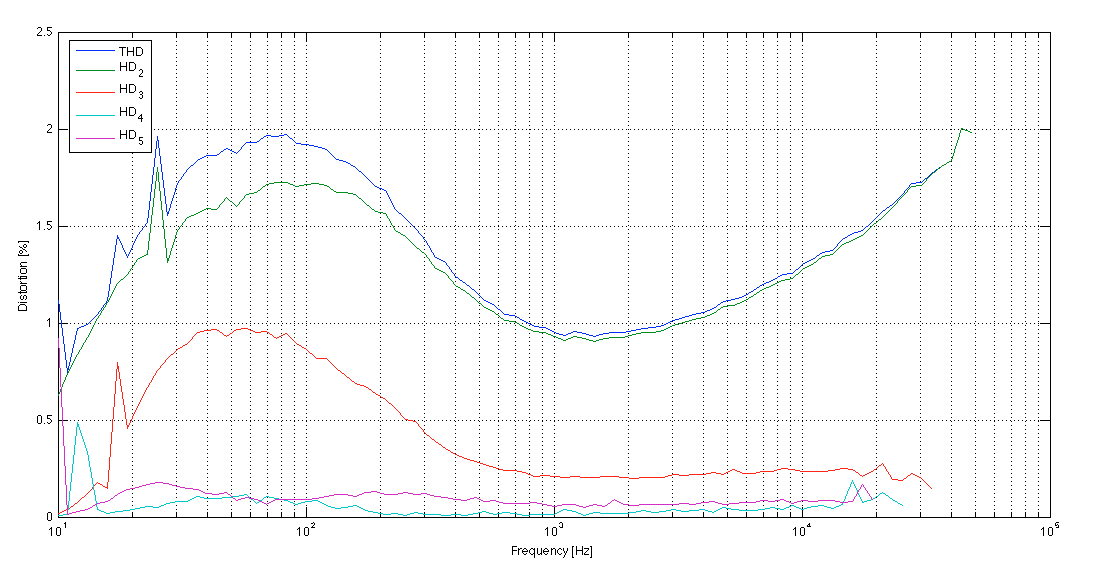
\includegraphics[width=\textwidth]{maalerapporter/final/mic/final_mic_3,16mv_thd.png}
\caption{Målt THD for HiFi-forstærkeren ved mikrofonindgang og 200 mV}
\label{maalerapport_final1}
\end{figure}

\begin{figure}[h]
\centering
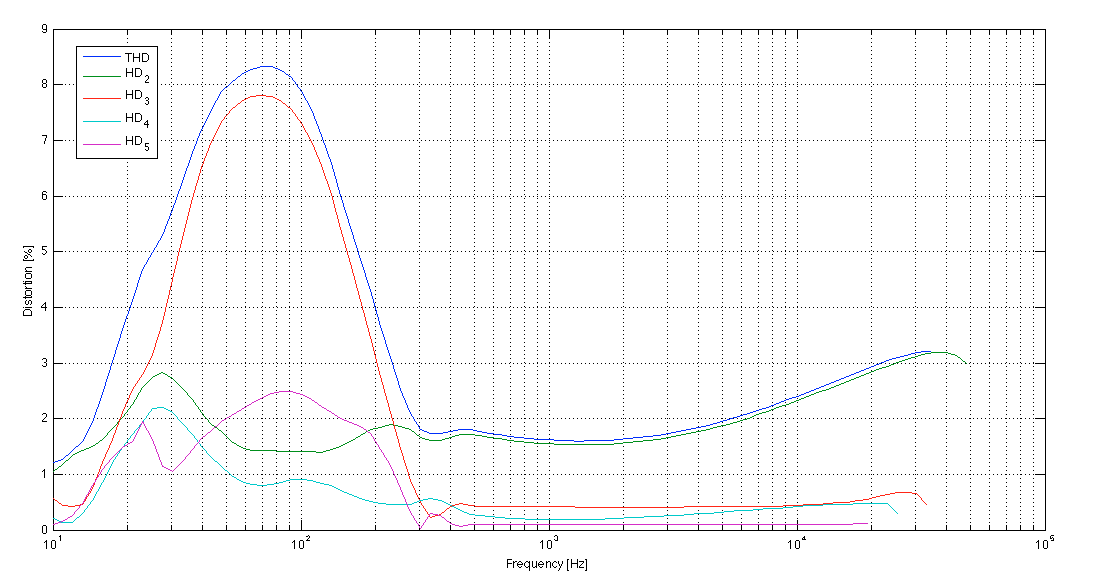
\includegraphics[width=\textwidth]{maalerapporter/final/mic/final_mic_31,6mv_thd.png}
\caption{Målt THD for HiFi-forstærkeren ved mikrofonindgang og 2 V}
\label{maalerapport_final2}
\end{figure}

\begin{figure}[h]
\centering
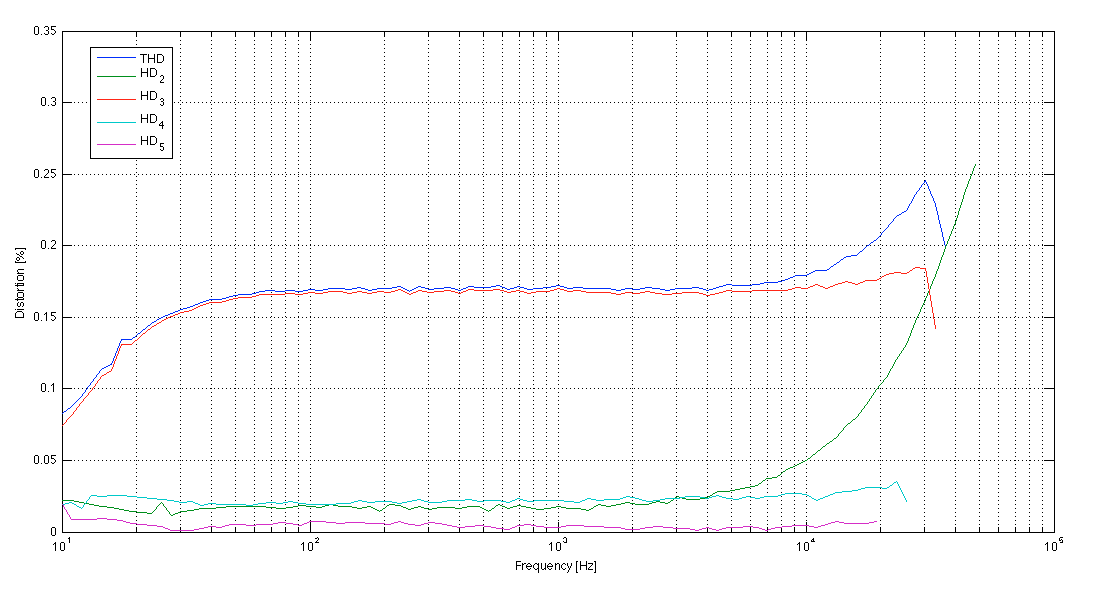
\includegraphics[width=\textwidth]{maalerapporter/final/stereo/final_stereo_200mv_thd.png}
\caption{Målt THD for HiFi-forstærkeren ved stereo indgang og 200 mV}
\label{maalerapport_final3}
\end{figure}

\begin{figure}[h]
\centering
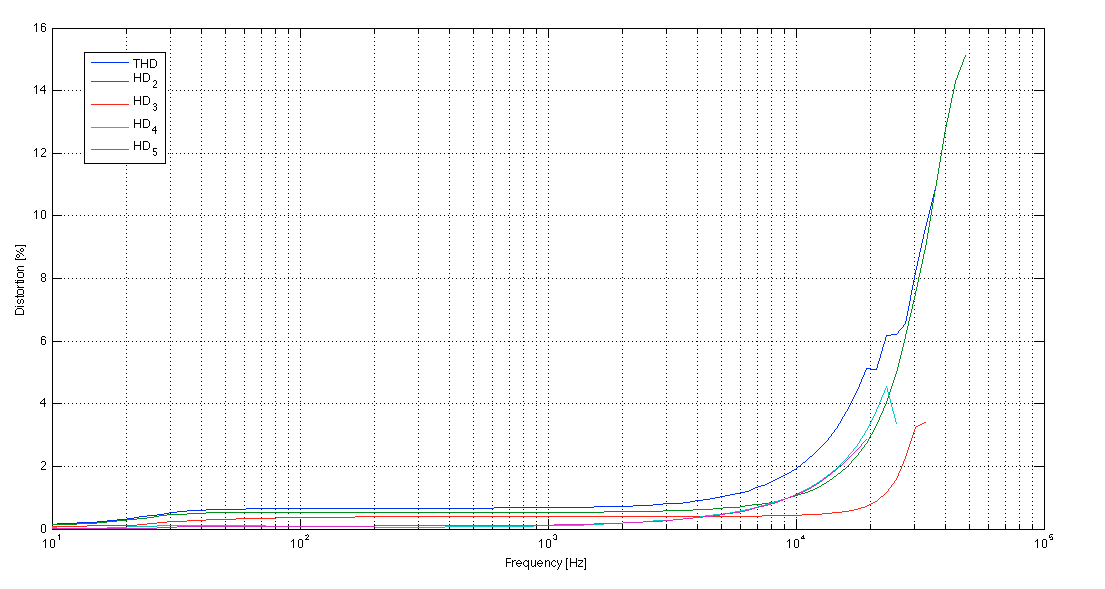
\includegraphics[width=\textwidth]{maalerapporter/final/stereo/final_stereo_2v_thd.png}
\caption{Målt THD for HiFi-forstærkeren ved stereo indgang og 2 V}
\label{maalerapport_final4}
\end{figure}

\begin{figure}[h]
\centering
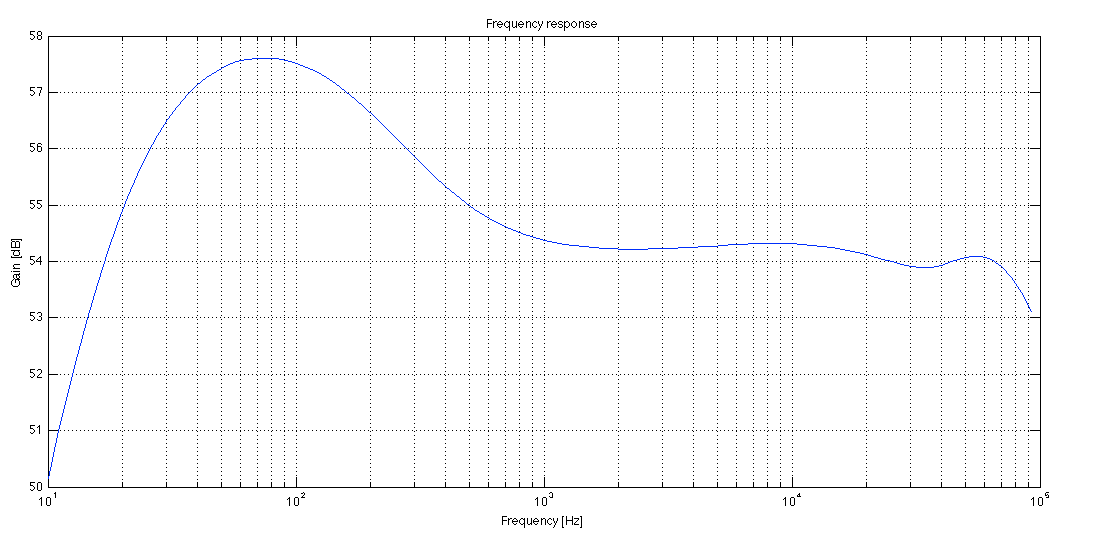
\includegraphics[width=\textwidth]{maalerapporter/final/mic/final_mic_3,16mv_frekvensgang.png}
\caption{Målt frekvensgang for HiFi-forstærkeren ved mikrofonindgang og 200 mV}
\label{maalerapport_final5}
\end{figure}

\begin{figure}[h]
\centering
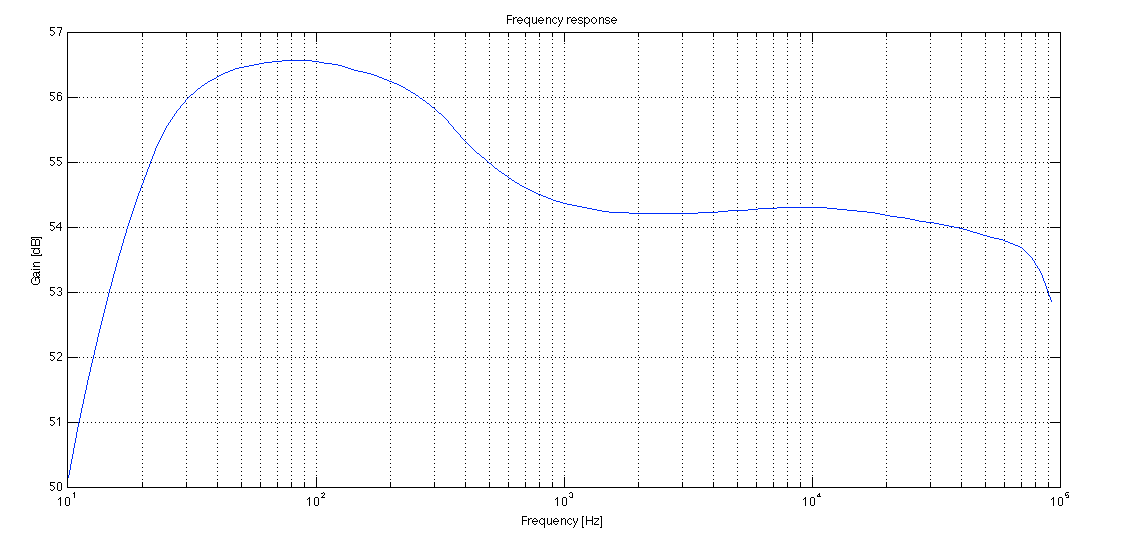
\includegraphics[width=\textwidth]{maalerapporter/final/mic/final_mic_31,6mv_frekevensgang.png}
\caption{Målt frekvensgang for HiFi-forstærkeren ved mikrofonindgang og 2 V}
\label{maalerapport_final6}
\end{figure}

\begin{figure}[h]
\centering
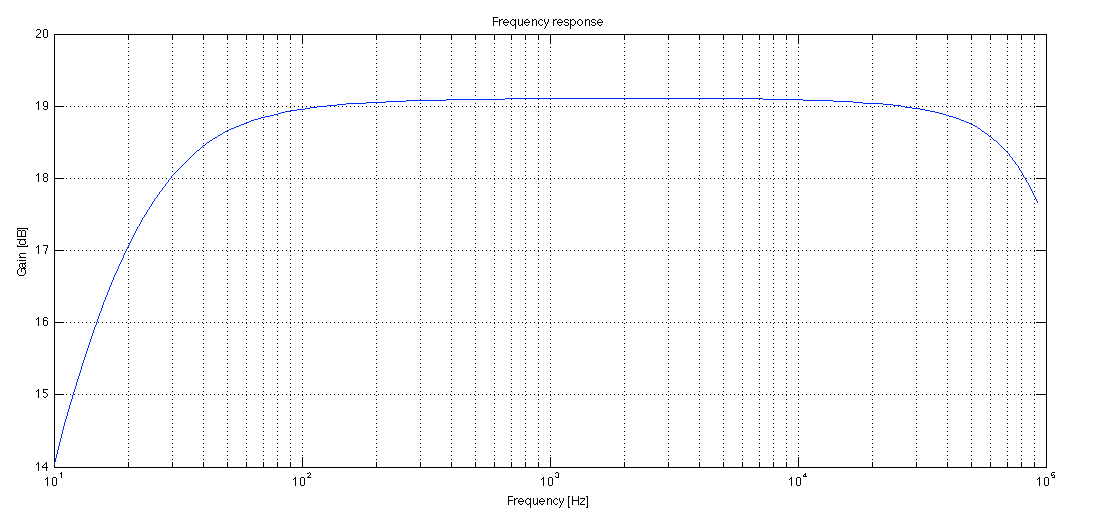
\includegraphics[width=\textwidth]{maalerapporter/final/stereo/final_stereo_200mv_frekvensgang.png}
\caption{Målt frekvensgang for HiFi-forstærkeren ved stereo indgang og 200 mV}
\label{maalerapport_final7}
\end{figure}

\begin{figure}[h]
\centering
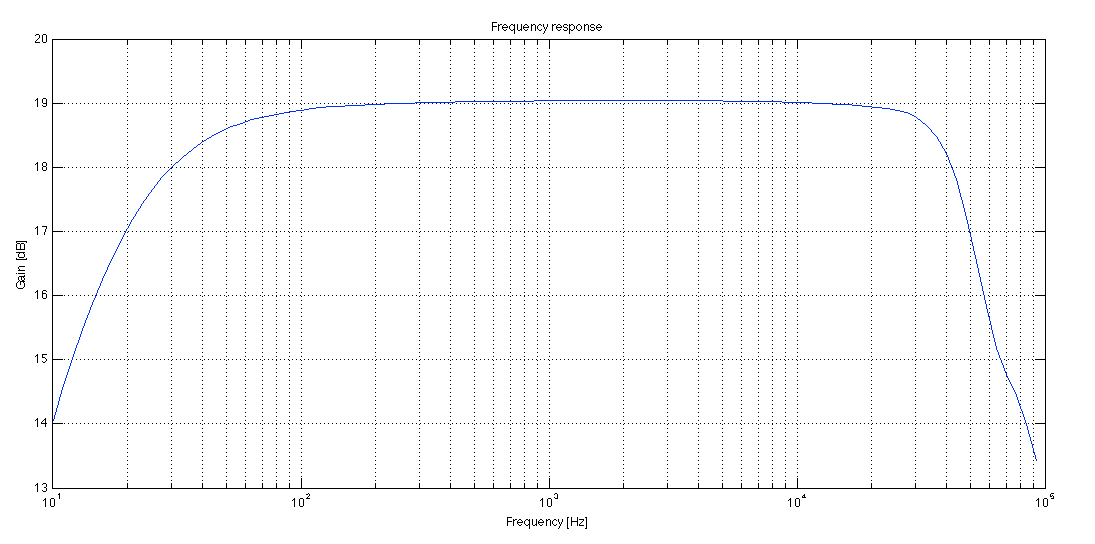
\includegraphics[width=\textwidth]{maalerapporter/final/stereo/final_stereo_2v_frekvensgang.png}
\caption{Målt frekvensgang for HiFi-forstærkeren ved stereo indgang og 2 V}
\label{maalerapport_final8}
\end{figure}